\documentclass{article}
\usepackage{tikz}
\usetikzlibrary{calc}
\begin{document}

\section{Tile serialized layout}
Please note that a full map has 398 'rows (i)', not just 6.

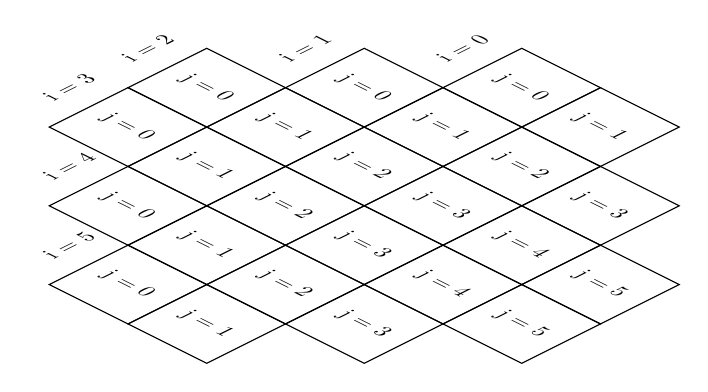
\begin{tikzpicture}[tile/.style = {rectangle,draw,yscale=.5,rotate=-45, minimum size = 14.14214mm},]

\node[tile] at (0,0) {j = 0};
\node[tile] at (1, -.5) {j = 1};

\node[tile] at (-2, 0) {j = 0};
\node[tile] at (-1, -.5) {j = 1};
\node[tile] at (0, -1) {j = 2};
\node[tile] at (1, -1.5) {j = 3};

\node[tile] at (-4, 0) {j = 0};
\node[tile] at (-3, -.5) {j = 1};
\node[tile] at (-2, -1) {j = 2};
\node[tile] at (-1, -1.5) {j = 3};
\node[tile] at (0, -2) {j = 4};
\node[tile] at (1, -2.5) {j = 5};

\node[tile] at (-5, -.5) {j = 0};
\node[tile] at (-4, -1) {j = 1};
\node[tile] at (-3, -1.5) {j = 2};
\node[tile] at (-2, -2) {j = 3};
\node[tile] at (-1, -2.5) {j = 4};
\node[tile] at (0, -3) {j = 5};

\node[tile] at (-5, -1.5) {j = 0};
\node[tile] at (-4, -2) {j = 1};
\node[tile] at (-3, -2.5) {j = 2};
\node[tile] at (-2, -3) {j = 3};

\node[tile] at (-5,-2.5) {j = 0};
\node[tile] at (-4, -3) {j = 1};

\node[rectangle, yscale=.5, rotate=45] at (-.75, .5) {i = 0};
\node[rectangle, yscale=.5,rotate=45] at (-2.75, .5) {i = 1};
\node[rectangle, yscale=.5,rotate=45] at (-4.75, .5) {i = 2};
\node[rectangle, yscale=.5,rotate=45] at (-5.75, 0) {i = 3};
\node[rectangle, yscale=.5,rotate=45] at (-5.75, -1) {i = 4};
\node[rectangle, yscale=.5,rotate=45] at (-5.75, -2) {i = 5};


\end{tikzpicture}

\section{Tile game layout}
Please note that a full map has 400 'rows (i)', not just 6.

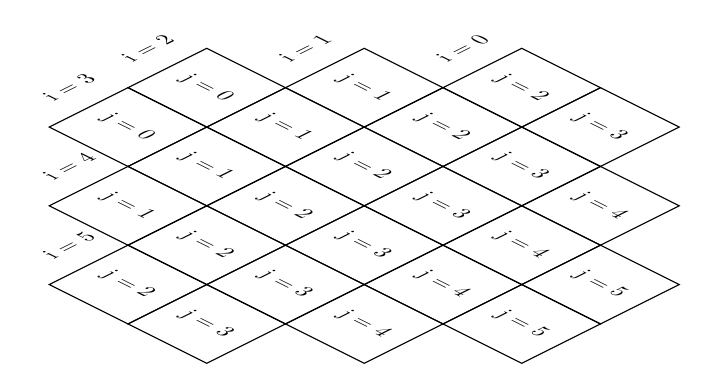
\begin{tikzpicture}[tile/.style = {rectangle,draw,yscale=.5,rotate=-45, minimum size = 14.14214mm}]

\node[tile] at (0,0) {j = 2};
\node[tile] at (1, -.5) {j = 3};

\node[tile] at (-2, 0) {j = 1};
\node[tile] at (-1, -.5) {j = 2};
\node[tile] at (0, -1) {j = 3};
\node[tile] at (1, -1.5) {j = 4};

\node[tile] at (-4, 0) {j = 0};
\node[tile] at (-3, -.5) {j = 1};
\node[tile] at (-2, -1) {j = 2};
\node[tile] at (-1, -1.5) {j = 3};
\node[tile] at (0, -2) {j = 4};
\node[tile] at (1, -2.5) {j = 5};

\node[tile] at (-5, -.5) {j = 0};
\node[tile] at (-4, -1) {j = 1};
\node[tile] at (-3, -1.5) {j = 2};
\node[tile] at (-2, -2) {j = 3};
\node[tile] at (-1, -2.5) {j = 4};
\node[tile] at (0, -3) {j = 5};

\node[tile] at (-5, -1.5) {j = 1};
\node[tile] at (-4, -2) {j = 2};
\node[tile] at (-3, -2.5) {j = 3};
\node[tile] at (-2, -3) {j = 4};

\node[tile] at (-5,-2.5) {j = 2};
\node[tile] at (-4, -3) {j = 3};

\node[rectangle, yscale=.5, rotate=45] at (-.75, .5) {i = 0};
\node[rectangle, yscale=.5,rotate=45] at (-2.75, .5) {i = 1};
\node[rectangle, yscale=.5,rotate=45] at (-4.75, .5) {i = 2};
\node[rectangle, yscale=.5,rotate=45] at (-5.75, 0) {i = 3};
\node[rectangle, yscale=.5,rotate=45] at (-5.75, -1) {i = 4};
\node[rectangle, yscale=.5,rotate=45] at (-5.75, -2) {i = 5};


\end{tikzpicture}

\section{Translation of coordinates}
Please note that a full map has 400 'rows (i)', not just 6.

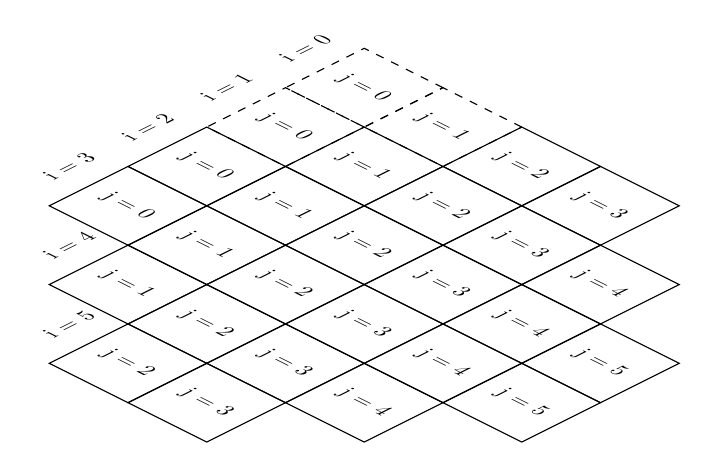
\begin{tikzpicture}[tile/.style = {rectangle,draw,yscale=.5,rotate=-45, minimum size = 14.14214mm},
			fictionaltile/.style = {rectangle,draw,dashed,yscale=.5,rotate=-45, minimum size = 14.14214mm}]

\node[fictionaltile] at (-2,1) {j = 0};
\node[fictionaltile] at (-1,0.5) {j = 1};

\node[tile] at (0,0) {j = 2};
\node[tile] at (1, -.5) {j = 3};

\node[fictionaltile] at (-3,0.5) {j = 0};
\node[tile] at (-2, 0) {j = 1};
\node[tile] at (-1, -.5) {j = 2};
\node[tile] at (0, -1) {j = 3};
\node[tile] at (1, -1.5) {j = 4};

\node[tile] at (-4, 0) {j = 0};
\node[tile] at (-3, -.5) {j = 1};
\node[tile] at (-2, -1) {j = 2};
\node[tile] at (-1, -1.5) {j = 3};
\node[tile] at (0, -2) {j = 4};
\node[tile] at (1, -2.5) {j = 5};

\node[tile] at (-5, -.5) {j = 0};
\node[tile] at (-4, -1) {j = 1};
\node[tile] at (-3, -1.5) {j = 2};
\node[tile] at (-2, -2) {j = 3};
\node[tile] at (-1, -2.5) {j = 4};
\node[tile] at (0, -3) {j = 5};

\node[tile] at (-5, -1.5) {j = 1};
\node[tile] at (-4, -2) {j = 2};
\node[tile] at (-3, -2.5) {j = 3};
\node[tile] at (-2, -3) {j = 4};

\node[tile] at (-5,-2.5) {j = 2};
\node[tile] at (-4, -3) {j = 3};

\node[rectangle, yscale=.5, rotate=45] at (-2.75, 1.5) {i = 0};
\node[rectangle, yscale=.5,rotate=45] at (-3.75, 1) {i = 1};
\node[rectangle, yscale=.5,rotate=45] at (-4.75, .5) {i = 2};
\node[rectangle, yscale=.5,rotate=45] at (-5.75, 0) {i = 3};
\node[rectangle, yscale=.5,rotate=45] at (-5.75, -1) {i = 4};
\node[rectangle, yscale=.5,rotate=45] at (-5.75, -2) {i = 5};


\end{tikzpicture}

\end{document}